\subsection{Nordöstliches Kongobecken}\label{sec:NordCongo}

\begin{figure*}[!tb]
	\centering
	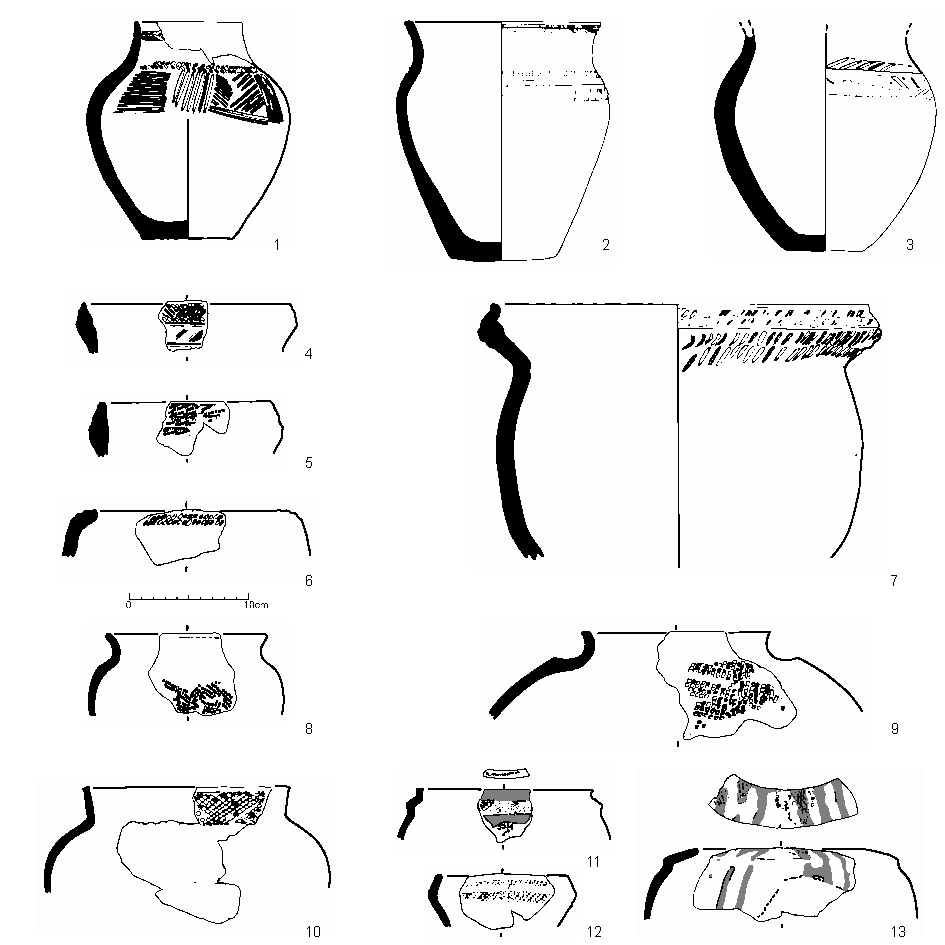
\includegraphics[width = \textwidth]{fig/neCongo_Typen.pdf}
	\caption{Nordöstliches Kongobecken: Regionale Sequenz nach \textcite{LivingstoneSmith.2017}.\\ 1--3: \textit{Ältere Phase} (\textit{cf}. Bomane Yangwa; nach ebd. 112 Abb. 24.2--4); 4--7: \textit{Mittlerer Phase} (\textit{cf}. Ilambi Moke; nach ebd. 113 Abb. 25.3, 25.1, 25.2, 25.8); 8--9: Ilambi-Gruppe (nach ebd. 113 Abb.~26.5, 26.1); 10--12: Yaekela-Gruppe (nach ebd. 114 Abb.~27.1, 27.6, 27.2); 13 Nkomba-Gruppe (nach ebd. 114 Abb.~28.1).}
	\label{fig:LivingstoneSmith2017_noCongoTrad}
\end{figure*}

Im Zuge des \textit{Boyekoli Ebale Congo}-Projekts wurden 2010 die unteren Abschnitte der Flüsse Lomami, Itimbiri und Aruwimi sowie 2013 des Lindi im nordöstlichen Kongobecken erstmals archäologisch untersucht \parencite[96]{LivingstoneSmith.2017}.\footnote{Die Ziele des \textit{Boyekoli Ebale Congo}-Projekts des \textit{Musée royal de l'Afrique centrale} in Tervuren (MRAC), des \textit{Institut royal des Sciences naturelles de Belgique} (IrSnB) und des \textit{Jardin botanique Meise} sowie der Universität Kinshasa (UNIKIN) lagen in der Untersuchung der Biodiversität entlang des Kongo. Zwischen dem 26.\,04.\,2010 und 26.\,06.\,2010 wurden drei große Zuflüsse des Kongo in seinem nördlichsten Bereich befahren. Die Forschungsmannschaft setzte sich aus 67 Wissenschaftlern der Fachbereiche Zoologie, Botanik, Hydrologie, Geologie, Kartografie, Archäologie und Linguistik zusammen (siehe \url{http://www.congobiodiv.org/en/projects/expeditions/expedition-2010} [Stand 17.\,05.\,2017]). Eine weitere, rein archäologische Untersuchung erfolgte zwischen dem 22.\,01.\,2013 bis 22.\,02.\,2013 \parencites[siehe][]{LivingstoneSmith.2011}{Cornelissen.2013}.\label{ftn:BoyekoliEbaleCongo}} Im Zuge der einzelnen Maßnahmen konnten insgesamt 14 Befunde an acht unterschiedlichen Fundstellen ausgegraben und dokumentiert werden \parencite[98 Tab.~1]{LivingstoneSmith.2017}. Eine in Bomane Yangwa am unteren Aruwimi untersuchte Grube (YNG/10/II) weist starke Ähnlichkeiten zu den Keramikdeponierungen des Inneren Kongobeckens auf \parencites[13 Abb.~2]{LivingstoneSmith.2011}[siehe][]{Wotzka.1993}. Der zirka 0,8\,m tiefe Befund weist eine stark mit kompletten Gefäßen oder Gefäßfragmenten \parencites[siehe][14 Abb.~3]{LivingstoneSmith.2011}[112 Abb.~24.4]{LivingstoneSmith.2017} durchsetzte innere Verfüllung auf, während eine diesen Bereich umgebende äußere Zone kaum Funde enthielt. Eine im unteren Bereich der an Gefäßfragmenten reichen inneren Verfüllung entnommene Radiokohlenstoffdatierung stellt den Befund in das 4.--1. Jh. v.~Chr. (ebd. 98 Tab.~1: Poz-39122). Eine ebenfalls in das 4.--1. Jh. v.~Chr. datierende Grube (ebd. 98 Tab.~1: Poz-57246, Poz-57248) fand sich in Baombi~II am Lindi (BAO/13/I; ebd. 101\,f.). Das keramische Fundgut, das ebenfalls aus großen, eng gepackten Gefäßteilen besteht (ebd. 102 Abb.~10, 18 Abb.~24.5), entspricht formal jenem aus Bomane Yangwa. Beide Inventare sowie Funde aus Ilambi Moke und Yandjambi am Lomami spiegeln zusammen die älteste von drei Hauptphasen wider, die durch diese ersten Feldarbeiten im nordöstlichen Kongobecken herausgearbeitet werden konnten (ebd. 110--112). Die Keramik dieser ältesten Phase zeichnet sich durch langovale Grundformen mit konvexen Schulterbereichen und flachen Standböden sowie einer Verzierung im Schulterbereich der Gefäße aus, das aus horizontalen Bändern aus Rillen in Zickzack- oder Fischgrät-Muster (Tab.~\ref{tab:Verzierungselemente}: 01.6--8) sowie Kammwiegeband (Tab.~\ref{tab:Verzierungselemente}: 04.1) besteht (ebd. 111 Abb.~23, 18 Abb.~24). Die Keramik weist häufig Schamott-Magerung auf und Makrospuren deuten auf eine Herstellung durch Treiben hin (ebd. 110--112). Die entsprechenden Merkmale werden von \textsc{\mbox{Livingstone} \mbox{Smith}} (ebd. 110) unter Vorbehalt mit der etwa zeitgleichen Keramik der Imbonga-Gruppe des Inneren Kongobeckens \parencite[59--68]{Wotzka.1995} in Zusammenhang gebracht. Es muss darauf hingewiesen werden, dass die Keramik der ältesten Phase des nordöstlichen Kongobeckens jedoch eher formale Ähnlichkeiten zu der im Zuge dieser Arbeit erstmals beschriebenen \mbox{Ngbanja}-Keramik aufweist (Kap.~\ref{sec:NGB-Gr} mit Abb.~\ref{fig:NGB_Typverteter}). Gerade die langovalen Grundformen und der Fokus der Verzierungen auf horizontale Bänder im Schulterbereich, wobei die Gefäßunterteile frei von Verzierungen sind, finden sich eher bei der frühen Keramik des mittleren \mbox{Ubangi} als in der Imbonga-Keramik des Inneren Kongbeckens, deren Gefäßunterteile und Standflächen systematisch mit Kamm-Wiegeband verziert sind (ebd. 65). Auch die für die Imbonga-Keramik typischen plastischen Verzierungselemente finden sich in dem von \textcite[112 Abb.~24]{LivingstoneSmith.2017} präsentierten Material nicht.\footnote{Einzelne aus dem Inneren Kongobecken stammende Keramikobjekte können unter Vorbehalt als potenzielle Vergleiche für das Material der älteren Phase des nordöstlichen Kongobeckens herangezogen werden. Insbesondere der Standringboden eines Gefäßes aus Bomane Yangwa \parencites[14 Abb.~3]{LivingstoneSmith.2011} weist eine grundsätzliche Ähnlichkeit zu Gefäßen der Imbonga-Gruppe aus Bokele (Fpl.~14), Bokuma (Fpl.~18) sowie Imbonga (Fpl.~43) auf \parencite[453 Taf.~19.4, 6, 9, 470 Taf.~36.12, 471 Taf.~37.7, 490 Taf.~56.2]{Wotzka.1995}.} Aufgrund von fünf Radiokohlenstoffdatierungen wird das keramische Material der ältesten Phase von \textcite[111 Abb.~23]{LivingstoneSmith.2017} hinreichend sicher in das 4. Jh. v.~Chr. bis 1.~Jh. n.~Chr. datiert.

An dieses Material schließen sich -- basierend auf den vorliegenden Datierungen -- formal andersartige Gefäße an, die einer in das 1. bis frühe 5. Jh. n.~Chr. datierenden mittleren Phasen zugerechnet werden (ebd. 111 Abb.~23). Die entsprechenden Stücke zeichnen sich durch höhere Anteile von Quarz und in wenigen Fällen auch Schamott im Scherben sowie Gefäßformen mit deutlich geschweifter Wandung aus (ebd. 110, 113 Abb.~25). Auffällig sind abgesetzte Schulterbereiche und ausgedünnte Ränder. Die Verzierungen bestehen vornehmlich aus in Wiegetechnik erzeugten Bändern (Tab.~\ref{tab:Verzierungselemente}: 04.1--2) und verschiedenen Eindrücken mit einzinkigen Geräten oder Kämmen. Entsprechende Funde lassen sich stromab noch bis in die Nähe von Lisala beobachten.\footnote{Eine Randscherbe mit ausbiegendem Rand und einbiegender Randlippe, die mit Kammwiegeband verziert ist und der mittleren, von Livingstone Smith u.\,a. (2017, 110\,f., 113 Abb.~25.8) beschriebenen keramischen Phase zugerechnet werden kann, findet sich in den Beständen der \textit{Musées Universitaires des Départements de Préhistoires et d'Archéologie de l'Université de Kinshasa} (UNIKIN; siehe Anm.~\ref{ftn:IleMimosas}).} Mit Ausnahme leichter Ähnlichkeiten der Randgestaltung der Bokonongo-Keramik (Kap.~\ref{sec:BOG-Gr}) des südlichen Teils des Arbeitsgebiets, lassen sich keine Parallelen zu gegenwärtig bekannten Stilgruppen erkennen.

Für die nachfolgenden keramischen Ausprägungen der späten Phase liegen lediglich zwei aus Yangambi stammende Radiokohlenstoffdatierungen vor, eine in das 8.--10.~Jh. n.~Chr. datierende Probe, sowie ein deutlich jüngeres, das 15.--17.~Jh. n.~Chr. abdeckendes Datum (ebd. 98 Tab.~1: Poz-75462, Poz-75451). Beide Datierungen repräsentieren keramisches Material, welches der Stilgruppe Ilambi zugerechnet werden kann. Diese zeichnet sich durch dünnwandige Gefäße mit abknickenden Schulterbereichen und deutlich konkav ausbiegenden, ausgedünnten Rändern aus (ebd. 111). Verzierungen kommen in Form von Rillen und Kammeindrücken auf den Gefäß"-oberteilen vor. Alternativ finden sich Gefäße mit nicht verziertem Oberteil, deren Unterteile mit einer bislang nicht genau identifizierten Technik flächig verziert sind. Entweder handelt es sich um ein aus mehreren hölzernen Kernen bestehendes mit Schnur umwickeltes \mbox{Roulette} \parencite[101 Abb.~1.29]{LivingstoneSmith.2010b} oder Mattenabdruck \parencite[111, 113 Abb.~26]{LivingstoneSmith.2017}. Zur Keramik der Ilambi-Gruppe sind keine Vergleichsfunde aus dem Arbeitsgebiet bekannt. Ebenfalls der jüngeren Phase zuzurechnen sind die Formen der Yaekela-Gruppe, die sich durch ebenfalls dünnwandige Gefäße mit geschweiften Wandungen und Schultern sowie ausbiegenden Rändern und flach abgestrichenen Randlippen auszeichnet (ebd. 111, 114 Abb.~27). Innerhalb der Yaekela-Gruppe finden sich auch offene Formen mit leicht geschweiften oder abknickenden Wandungen, die ebenfalls flach abgestrichene Randlippen aufweisen. Die Verzierungen dieser Stilgruppe bestehen vornehmlich aus Schnitzroulette (siehe Tab.~\ref{tab:Verzierungselemente}: 21.7), das gelegentlich von Kammeindrücken eingerahmt wird. Ebenfalls beobachtet wurde die erstmals durch \textcite[207--210, 536 Taf.~102.2--4, 6--16]{Wotzka.1995} beschriebene Nkomba-Gruppe. Die Keramik dieser Stilgruppe zeichnet sich vor allem durch eine Bemalung aus umlaufenden oder unterbrochenen roten Streifen sowie begleitender Rillen- oder Riefenzier aus \parencite[114 Abb.~28]{LivingstoneSmith.2017}.\footnote{Vertreter dieser Stilgruppe, die von \textcite[223\,f.]{Wotzka.1995} als Teil einer von der keramischen Entwicklung des Inneren Kongobeckens unabhängigen \textit{Nord-Tradition} angesehen wurden, finden sich auch in der Vorlage ethnografischer Funde des ehemaligen \textit{Musée du Congo} \parencite[152--154, 157--159, Taf.~13.189--191]{Coart.1907}. Dies unterstreicht die subrezente Zeitstellung der Nkomba-Keramik. Siehe Kap.~\ref{sec:ICB_StilGrDatierungen}.} Allen Stilgruppen der späten Phase gemein sind innenseitige Abdrücke von Stempeln, die auf eine Herstellung durch Abformen in einer konkaven Form hinweisen \parencite[111]{LivingstoneSmith.2017}. Diese Technik wurde bislang weder im Inneren Kongobecken nachgewiesen und auch im Arbeitsgebiet findet sie sich lediglich im nördlichsten Bereich, entlang des oberen \mbox{Ubangi}.\footnote{Siehe Anm.~\ref{ftn:EthnoToepfereiInVorb}.} Die späte Phase repräsentiert somit einen deutlichen Bruch in der technologischen Tradition des von \textcite{LivingstoneSmith.2017} untersuchten Raumes: von in Aufbautechnik hergestellten und mittels Rillen, Riefen sowie Eindrücken verzierten Gefäßen in der vom 4. Jh. v.~Chr. bis 5. Jh. n.~Chr. reichenden frühen sowie mittleren Phase zu potenziell in Abformtechnik hergestellten und mittels \mbox{Roulette} verzierten jüngeren Stilen, die ab dem 8. Jh. n.~Chr. aufkommen.